\section{区间估计}

区间估计是统计学中一种常用的方法,用于估计一个参数的值在一个给定的区间内的范围.
在实际应用中,我们往往无法得到一个参数的精确值,而是通过收集样本数据,利用统计方法来估计这个参数的取值范围.

\subsection{区间估计的定义}

\begin{definition}[区间估计]
    设总体 $ X $ 的分布函数为 $ F(x ; \theta)$,含有未知参数 $ \theta \in \Theta$ ($\Theta $ 是 $ \theta $ 的取值范围),
    对于给定的 $ \alpha(0<\alpha<1), \underline{\theta}=\underline{\theta}\left(X_{1}, X_{2}, \cdots, X_{n}\right) $ 和 $ \bar{\theta}=\bar{\theta}\left(X_{1}, X_{2}, \cdots, X_{n}\right)(\underline{\theta}<\bar{\theta}) $
    是来自 $ X $ 的样本 $ X_{1}, X_{2}, \cdots, X_{n} $ 确定的两个统计量,若对于任意 $ \theta \in \Theta $ 满足
    $$P\left\{\underline{\theta}\left(X_{1}, X_{2}, \cdots, X_{n}\right)<\theta<\bar{\theta}\left(X_{1}, X_{2}, \cdots, X_{n}\right)\right\} \geqslant 1-\alpha$$
    则称随机区间 $ (\underline{\theta}, \bar{\theta}) $ 为\textit{参数} $ \theta $ \textit{的置信水平为} $ 1-\alpha $ \textit{的置信区间},$\theta $ 和 $ \bar{\theta} $
    分别称为\textit{置信水平为} $ 1-\alpha $ 的双侧置信区间的\textit{置信下限}和\textit{置信上限},$1-\alpha $ 称为\textit{置信水平}.
\end{definition}

置信水平 $ 1-\alpha $ 的含义: 在随机抽样中,若重复抽样多次 (每次的样本容量相同),
得到样本 $ X_{1}, X_{2}, \cdots, X_{n} $ 的多个样本值,对应每个样本值都确定了一个置信区间 $ (\underline{\theta}, \bar{\theta}) $,
每个这样的置信区间要么包含了 $ \theta $ 的真值,要么不包含 $ \theta $ 的真值.

根据伯努利大数定理,当抽样次数充分大时,这些置信区间中包含 $ \theta $ 的真值的频率接近于置信水平 (即概率) $ 1-\alpha $,
即在这些置信区间中包含 $ \theta $ 的真值的置信区间大约有 $ (1-\alpha) \times 100 \% $ 个,
不包含 $ \theta $ 的真值的置信区间大约有 $ \alpha \times 100 \% $ 个.
例如,给定 $ \alpha=0.05 $,则置信水平是 $0.95$,若重复抽样 $10000$ 次,对应每次抽样都确定了一个置信区间 $ (\underline{\theta}, \bar{\theta}) $,
则其中大约有 $9500$ 个置信区间包含 $ \theta $ 的真值,大约有 $500$ 个置信区间不包含 $ \theta $ 的真值.
也就是说,某一置信区间中包含 $ \theta $ 的真值的概率是 $0.95$.

\begin{example}
    已知某种袋装食盐的质量 $ X $ 服从正态分布 $ N\left(\mu, \sigma^{2}\right)$,
    从一批食盐中随机抽取 $9$ 袋,测得其质量 (单位: $ g $) 分别为
    $$\begin{array}{lllllllll}
            502 & 503 & 501 & 503 & 498 & 502 & 499 & 500 & 501
        \end{array}$$
    已知 $ \sigma=1 $,求总体均值 $ \mu $ 的置信水平为 $0.95$ 的置信区间.
\end{example}
\begin{solution}
    由于统计量 $Z=\dfrac{\bar{X}-\mu}{\sigma/\sqrt{n}}\sim N(0,1)$,按标准正态分布上 $\alpha$ 分位点的定义 (见图 \ref{alphafweidian}),
    有 $$P\qty{\qty|\dfrac{\bar{X}-\mu}{\sigma/\sqrt{n}}|<z_{\alpha/2}}=1-\alpha$$
    即 $$P\qty{\bar{X}-z_{\alpha/2}\sigma/\sqrt{n}<\mu<\bar{X}+z_{\alpha/2}\sigma/\sqrt{n}}=1-\alpha$$
    故此置信区间为
    \begin{equation}
        \qty(\bar{X}-z_{\alpha/2}\sigma/\sqrt{n},\bar{X}+z_{\alpha/2}\sigma/\sqrt{n})
        \tag{1}
    \end{equation}
    常缩写为 $\qty(\bar{X}\pm z_{\alpha/2}\sigma/\sqrt{n})$.
\end{solution}

\begin{figure}[H]
    \centering
    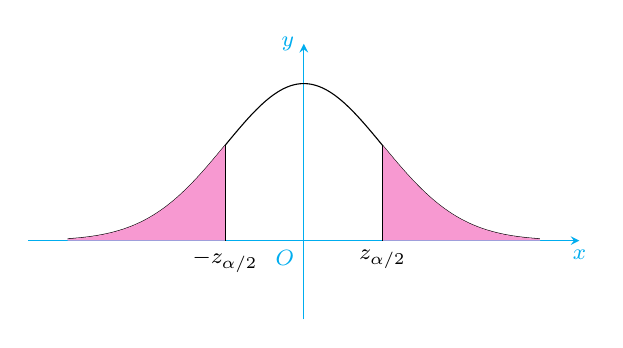
\begin{tikzpicture}[->,samples=100,>=stealth,font=\footnotesize,yscale=5]
        \def\xmin{-3.5}
        \def\xmax{3.5}
        \def\ymin{-.2}
        \def\ymax{.5}
        \def\a{0.398942}
        \draw[->,cyan](\xmin,0)--(0,0)node[below left]{$O$}--(\xmax,0)node[below]{$x$};
        \draw[->,cyan](0,\ymin)--(0,\ymax)node[left]{$y$};

        \draw[scale=1,domain=-3:3,smooth,variable=\x,black,-] plot ({\x},{\a*exp(-\x*\x/2)});

        \fill[color=magenta!40] (1,0) -- plot[domain=1:3,smooth,variable=\x] ({\x},{\a*exp(-\x*\x/2)}) -- (3,0) --cycle;
        \node[below] at (1,0) {$z_{\alpha/2}$};
        \draw[-] (1,0)--plot[domain=1:1,smooth,variable=\x] ({\x},{\a*exp(-\x*\x/2)});

        \fill[color=magenta!40] (-1,0) -- plot[domain=-1:-3,smooth,variable=\x] ({\x},{\a*exp(-\x*\x/2)}) -- (-3,0) --cycle;
        \node[below] at (-1,0) {$-z_{\alpha/2}$};
        \draw[-] (-1,0)--plot[domain=-1:-1,smooth,variable=\x] ({\x},{\a*exp(-\x*\x/2)});
    \end{tikzpicture}
    \caption{}
    \label{alphafweidian}
\end{figure}

由于 $ \alpha=0.05$,查表知 $ z_{0.025}=1.96$,
且由于 $ \sigma=1, n=9, \bar{x}=501 $,由式 (1),
得到 $ \mu $ 的置信水平为 $0.95$ 的置信区间为 $\qty(501 \pm 1.96 \times 1 / \sqrt{9}) $,即  $(500.35,501.65)$ .

这个区间的含义是: 若反复抽样多次,每次抽样均确定一个置信区间,在这些置信区间中,包含 $ \mu $ 的约占 $ 95 \% $,
或者说某一置信区间是包含 $ \mu $ 的区间的可信程度为 $ 95 \% $.
置信区间长度的一半是 $0.65$,表示用 $ \bar{x}=501 $ 来估计参数 $ \mu $ 的误差不大于 $0.65$,这个误差估计的可信程度是 $ 95 \% .$

若给定置信水平 $0.99$ 时,则 $ \alpha=0.01$,查表知 $ z_{0.005}=2.58$,
得到置信区间为 $ (500.14 , 501. 86)$. 可以看出,当给定的置信水平越大时,即 $ 1-\alpha $ 越大,
则 $ \alpha $ 值越小,$z_{\alpha / 2} $ 越大,从而置信区间长度 $\displaystyle 2 z_{\alpha / 2} \frac{\sigma}{\sqrt{n}} $ 越大,
参数估计的精确程度越差.

\subsection{区间估计的一般步骤}

求置信区间的基本步骤如下:
\begin{enumerate}[label=(\arabic{*})]
    \item 选择一个与样本 $ X_{1}, X_{2}, \cdots, X_{n} $ 及 $ \theta $ 有关的函数 $ W\left(X_{1}, X_{2}, \cdots, X_{n} ; \theta\right) $,
          使得 $ W $的分布不依赖于 $ \theta $ 和其他未知参数,称具有这种性质的函数 $ W $ 为枢轴量.
          枢轴量选取的标准为:
          \begin{enumerate}
              \item 必须含有要估计的参数 $ \theta $,不含有其他未知参数;
              \item 尽量使用总体的已知信息.
          \end{enumerate}
    \item 对于给定的置信水平 $ 1-\alpha$,根据 $\displaystyle P\left\{a<W\left(X_{1}, X_{2}, \cdots, X_{n} ; \theta\right)<b\right\}=1-\alpha $,
          在枢轴量 $ W $ 为常用分布的情况下,$a$ 和 $ b $ 可由分位数表查得.

          选择分位数 $ a $ 和 $ b $ 的标准是使区间 $ (a, b) $ 最小,实际应用中很难实现这一点,因此通常选取 $ a $ 和 $ b $ 使得
          $\displaystyle P\left\{W\left(X_{1}, X_{2}, \cdots, X_{n} ; \theta\right) \leqslant a\right\}=P\left\{W\left(X_{1}, X_{2}, \cdots, X_{n} ; \theta\right) \geqslant b\right\}=\alpha / 2 .$
    \item 由 $ a<W\left(X_{1}, X_{2}, \cdots, X_{n} ; \theta\right)<b$,作恒等变形后解出参数 $ \theta $ 的取值范围,即为所求的置信区间 $ (\underline{\theta}, \bar{\theta}) $.
    \item 代人已知样本数据进行计算.
\end{enumerate}
